\documentclass[onecolumn, 12pt]{article}
\usepackage{hyperref,mathtools,amssymb}
\usepackage{cite}
\usepackage{graphicx}
\usepackage{xcolor}
\usepackage{subcaption}
\usepackage[margin=0.75in]{geometry}

\title{ERCAP Proposal: rotating bosons via CL with AMReX}
%\subject{Many-Body Quantum Mechanics}
\author{Casey Berger, Don Willcox}
\date{\today}

\newcommand{\casey}[1]{{\color{green} \bf[CB: #1]}}
\newcommand{\don}[1]{{\color{blue} \bf[DW: #1]}}
\newcommand{\etal}{{\it et al.}}
\newcommand{\beq}{\begin{equation}}
\newcommand{\eeq}{\end{equation}}
\newcommand{\bea}{\begin{eqnarray}}
\newcommand{\eea}{\end{eqnarray}}

\newcommand{\MarginPar}[1]{\hspace{1sp}\marginpar{\tiny\sffamily\raggedright\hspace{1sp}{\color{blue}#1}}}

\def\CP{{\mathcal P}}
\def\CC{{\mathcal C}}
\def\CH{{\mathcal H}}
\def\CW{{\mathcal W}}
\def\CO{{\mathcal O}}
\def\CZ{{\mathcal Z}}
\def\CD{{\mathcal D}}
\def\del{{\nabla}}

\newcommand*\dif{\mathop{}\!\mathrm{d}}

\begin{document}
\section{Project Description}
TO DO
\begin{itemize} 
	\item DONE  - can be shortened
	
	Goals: Please summarize the area of research on which you?ll be working during the 30-day Early User Program, and any specific research or performance goals that you hope to achieve.
	
	\item IN PROGRESS -- need to emphasize use of GPUs
	
	Resource selection: Please summarize why you have selected these specific resources (e.g., Regular Memory, Extreme Memory, and/or GPU nodes, and storage) to achieve these scientific goals.

    {\color{blue} I've added some sentences to explain that we've put effort into using GPUs well and that has paid off with good performance that makes the Bridges-2 system ideal for this work.}
	
	\item Please confirm that your team agrees to provide feedback on the Early User Program, including a brief description of what you were able to achieve, near the conclusion of the 30-day Early User Program.

	{\color{blue} Added a sentence to the paragraph discussing performance.}
	
	\item Special considerations, if any (e.g., a need for VMs to support persistent web services or databases, interactive access to a large number of nodes, minimum of 2048 cores/job)
\end{itemize}
\subsection{Goals of the project}
This project aims to calculate properties of a rotating bosonic superfluid. Experimental study of superfluids under rotation have revealed the onset of quantized vortices with increasing rotational frequency, an example of macroscopic quantum behavior. Theoretical treatment of these systems struggles due to the presence of the ``sign problem," a challenge which plagues the study of many interesting quantum many-body systems. This project applies a method well-known in the community of lattice gauge theory, known as complex Langevin (CL), to circumvent the sign problem in the numerical study of a system of rotating, trapped, and interacting nonrelativistic bosons. 

Rotating bosonic systems can be described using the path-integral formulation:
%
\beq
\CZ = \int \dif \phi e^{-S[\phi]}
\eeq
%
with the action in $2+1$ dimensions given by
%
\beq
S = \int \dif x \dif y \dif\tau \left[ \phi^{*}\left( \partial_{\tau} - \frac{\del^{2}}{2m} - \mu  - \frac{m}{2} \omega_{\text{trap}}^{2}(x^{2}+y^{2})- i \omega_{z}(x \partial_{y} - y\partial_{x})\right)\phi + \lambda (\phi^{*} \phi)^{2}\right],
\eeq 
%
where our scalar fields are functions of space and euclidean time, $\phi(x,y,\tau)$. The bosonic fields are complex scalar fields, and the addition of a rotational term in the action makes the system irretrievably complex. In order to treat this action composed of complex-valued fields, we use the CL method.

Complex Langevin is a stochastic method for treating field-theoretical models with a complex action. It extends the well-established Langevin method to complex-valued fields, evolving those fields in a fictitious time called Langevin time, resulting in a set of field values distributed with the appropriate weight $e^{-S}$, from which quantities of interest can be computed via a simple statistical average. This treatment has been shown to be successful in toy models for finite quark density QCD~\cite{BergerCLReview} as well as in low energy atomic systems such as the polarized unitary Fermi gas~\cite{BergerCLReview}. 

I have developed and previously tested a code using CL to measure certain properties of this system. A sign problem emerges immediately in the formulation of the system with complex scalar fields, and CL has been shown to correctly reproduce known analytical solutions for simple versions of the system, i.e. with no rotation, external trap, or interaction. The code for this project is written in C++ and utilizes the AMReX framework. The adaptive mesh framework in AMReX will allow us to use a nonuniform mesh to calculate the field values, which enables more efficient use of computing resources. As the lattice size grows, we concentrate our resolution in the center of the lattice, where the interesting physics will be confined due to the presence of the harmonic traps, which reduce the presence of the fields rapidly to zero outside a narrow region in the center of the trap. Early work on this system with the additional features of rotation, trapping, and interaction have demonstrated the need to progress to significantly larger lattices in order to resolve the behavior of the rotating fluid on the lattice. Ultimately, we wish to produce calculations of quantized angular momentum and the density profiles of vortex formation in the fluid. 

To progress to the full system, it's essential to increase the computational resources in order to resolve much larger lattices. Scaling studies have been performed and tests have been done to elucidate the computational needs of this problem, and the results of these studies are discussed in Section~\ref{scaling}. We expect this work to result in multiple papers, as the application of this method to low-energy bosonic systems has been minimally studied in the past, and this work will result in insights into both the method and the system itself.

\section{Resource Selection and Computational Considerations}
\subsection{\label{scaling}Scaling and Performance}
This code uses AMReX, a high-performance AMR library developed at LBNL and funded as an ECP Co-Design Center. We use AMReX data structures to discretize the spacetime lattice upon which the fields are defined, distribute the lattice across MPI, and implement local parallelism for CPU, KNL, or GPU-based platforms while maintaining performance portability. 

While each step in Langevin time must be performed sequentially, the spacetime lattice can be updated at each of these Langevin steps in a naively parallel fashion. We divide the lattice into boxes (or grids) distributed across MPI ranks, so to advance the solution we first fill ghost cells throughout the domain to support the nearest neighbor sums that appear in the drift function. Next, we perform the drift function calculations and Langevin update - these are entirely local operations for each MPI rank. %We parallelize this local work using OpenMP with logical tiling for CPUs or KNL to maintain cache efficiency. 
When running on GPUs, we transparently launch CUDA kernels and disable logical tiling to ensure maximum kernel occupancy.

We also efficiently calculate observables at runtime, which requires summing terms across the entire lattice for density, field modulus, circulation, and other quantities of interest. On each MPI rank, the observables are first calculated for local grids 
%via OpenMP sum reductions (or 
using CUDA atomics. We then combine partial sums across the lattice using all-to-one MPI reductions. In Fig.~\ref{Fig:GPUScaling} we compare strong scaling curves on the Cori GPU development system for a $1024^3$ lattice for a run without observables (orange) and a run where we calculate observables every 10 Langevin steps (blue). We demonstrate that although the additional computation and communication for observables requires about twice as much walltime, our reduction strategy yields nearly ideal strong scaling efficiency.

Our parallel implementation uses AMReX abstractions developed for performance portability on heterogeneous architectures. We developed and tested it on the NERSC Cori GPU development platform. We have invested our development efforts in writing the local work loops to fully exploit the data-parallel portions of the CL algorithm that calculate drift functions and the CL lattice update. We also leverage the CUDA random number generation library for GPUs and have organized the observable computations into efficient GPU kernels. Our strategy has paid off with significant speedups - we run fully $150\times$ faster with MPI+CUDA on 96 NVIDIA V100 GPUs compared with MPI+OpenMP on 96 Xeon Phi CPU-based accelerators.
%We present scaling studies on Cori KNL in Fig.~\ref{Fig:KNLScaling} showing good strong scaling efficiency up to 10,000 KNL cores for a moderately sized domain of $512^3$ lattice sites.
In Fig.~\ref{Fig:GPUScaling} we also show excellent strong scaling on the Cori GPU test system using up to 96 GPUs for moderate and larger ($1024^3$) domains. Our development efforts and performance on GPUs make the Bridges-2 GPU nodes essential for efficiently running our proposed work, and we will share feedback on our achieved performance metrics and runtime configuration from this Early User Program with the Bridges-2 supercomputing team.

%
%\vspace{-3mm}
%\begin{figure}[h]
%\centering
%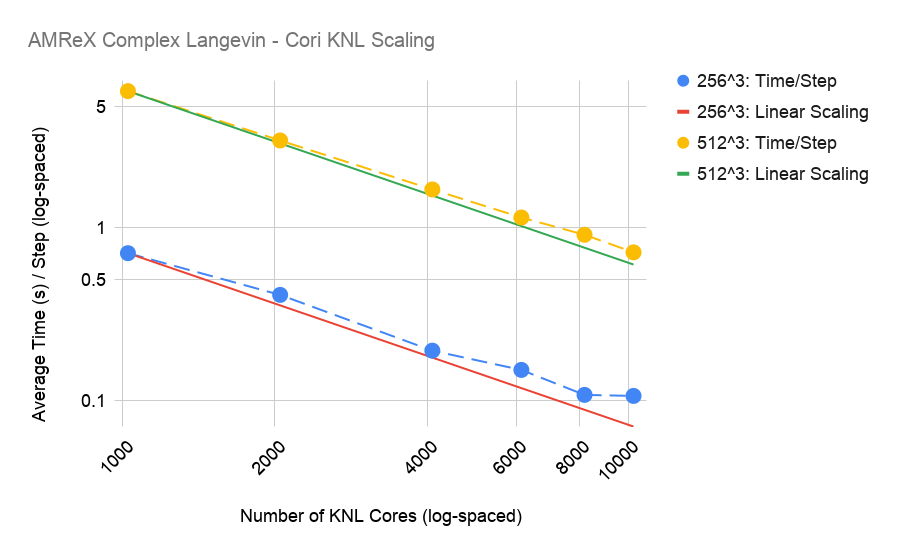
\includegraphics[width=0.6\textwidth]{./AMReX_Complex_Langevin_Cori_KNL_Scaling.png}
%\caption{\label{Fig:KNLScaling} Strong scaling for AMReX Complex Langevin on Knights Landing accelerators. These runs were performed with box sizes of $32^3$, 4 MPI tasks per node, and 16 OpenMP threads/MPI task.\vspace{-3mm}}
%\end{figure}
%\vspace{-3mm}
%

%
%\vspace{-3mm}
\begin{figure}[h]
\centering
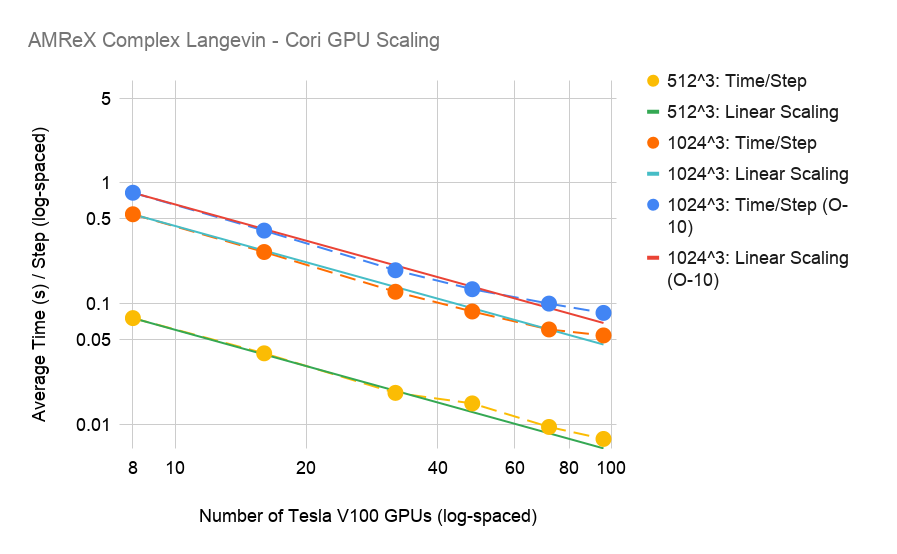
\includegraphics[width=0.6\textwidth]{./AMReX_Complex_Langevin_Cori_GPU_Scaling.png}
	\caption{\label{Fig:GPUScaling} Strong scaling for AMReX Complex Langevin on NVIDIA Tesla V100 GPUs. These runs were performed with box sizes of $32^3$ and $128^3$ for the $512^3$ and $1024^3$ domains, respectively, using 1 MPI task per GPU and no logical tiling. For the run labeled ``O-10'' we calculate observables every 10 Langevin steps, otherwise we turn off observables to measure performance for the Langevin advance alone.\vspace{-3mm}}
\end{figure}
%\vspace{-3mm}
%

Initially, some further testing will need to be done on these larger lattices in order to determine the correct balance of trapping frequency, lattice size, rotation frequency, and interaction strengths. Once these parameter values are set, we will need to collect on the order of one hundred data points on each lattice (varying the chemical potential and the rotation frequency), where each data point is collected by performing a Langevin evolution of $10^{6}$ steps on a full $N_{x} \times N_{x} \times N_{\tau}$ lattice. We also wish to extend our time domain and examine the effect of decreasing the temperature on the formation of vortices, which will include a run at a fixed set of parameters for multiple lattices of varying temporal extent. %Ultimately, we expect to need around 30 Mhr to complete this study with rigor.

\bibliography{XSEDEbib}{}
%\bibliographystyle{ieeetr}
\bibliographystyle{plain}
\end{document}
